\subsection{Depth-first search}

When traversing a graph, the same procedure happens over and over again:
\begin{itemize}
    \item choose a node;
    \item check that it has not been visited before;
    \item process the node;
    \item add its neighbours to the waiting list.
\end{itemize}

At the beginning, we add the starting point to the waiting list,
then we execute that procedure until the waiting list is empty.

If the graph is connected, it means we have traversed it entirely.
Otherwise, it means we have traversed one \emph{connected component}
of the graph, and we have to choose a new starting point.

\emph{Depth-first search}, or \emph{DFS}, uses a stack as waiting list.
The consequence is that as soon as a new node is discovered, it will be
explored, so depth-first search will progress quickly through the graph,
going in \emph{depth}
instead of exploring its most direct neighbourhood first.

The diagram below shows the order in which nodes are visited,
taking the example of a tree:
\begin{center}
    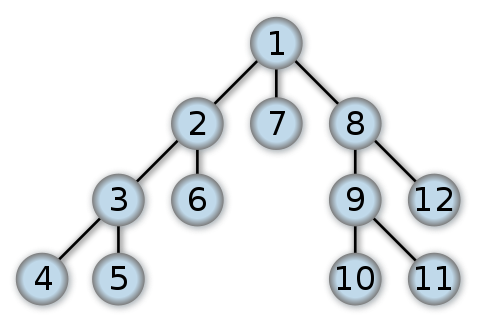
\includegraphics[width=0.3\textwidth]{img/dfs}
\end{center}

DFS can also be implemented with a recursive function:
instead of adding the neighbours to the waiting list, just calling the
visit procedure on them will have the same effect.
This may sound more simple, but internally it still uses the a stack,
the \emph{call stack}, that stores information about which functions
the program is in.

An interesting property is that the search never jumps from one side of the
graph to the other. After it has visited the first neighbour, the search only
has to go back to the original node through one edge,
then continue with the next neighbour.
In the above example, the path taken would be
$1,2,3,4,3,5,3,2,6,2,1,7,1,8,\ldots$
It goes through every edge exactly two times.

This makes it a viable option to physically traverse a graph (for example,
finding the center of a maze with loops, or exploring a cave system in
Minecraft) without having to remember anything, at the cost of a few markers.
